\subsection{Weigths}
\begin{figure}[t]
		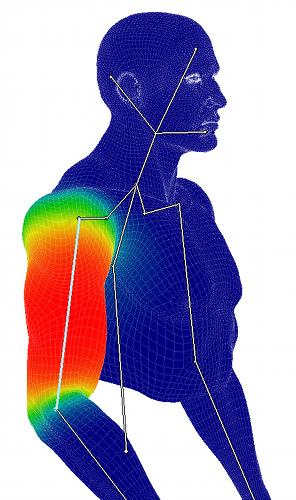
\includegraphics[width=7cm]{01_Skinning/pics/weight.png}
		\caption[Fl�chige Gewichtsverteilung]{ Modelldarstellung der fl�chigen Gewichtsverteilung auf einem Mesh. Die Farben beschreiben die Verteilung der Gewichte auf einer Skala von Blau=0, damit unabh�ngig, zu Rot=1, damit komplett abh�ngig. Entnommen von \cite{weights}}
		\label{weights_fig1}
\end{figure}

Gewichte bezeichnen wie abh�ngig ein Punkt auf dem Gittergraphen bei einer Transformation von einem Knochen ist. Sie sind die L�sung um bei verformbaren Material abzusch�tzen inwiefern sich jeder Punkt auf der Haut beeinflussen l�sst. Dieses Gewicht $wi$ in Relation zu Knochen $i$, ist $0<=wi<=1$. Wobei 0 komplett unabh�ngig von dem Knochen und 1 komplett von dem Knochen abh�ngig ist. So w�re zum Beispiel ein Punkt auf dem Oberarm des Knochen diesem komplett mit einer 1 zugeh�rig, ein Punkt an der H�fte h�tte ein Gewicht von 0 am Oberarm und w�re damit komplett unabh�ngig von diesem. Gewichte von Punkten am Ellbogengelenk h�tten variierende Werte zwischen 0 und 1. 

Nun k�nnten wir f�r jeden Vertex eine Liste erstellen mit allen seinen Gewichten in Bezug auf jedem Knochen, um zusammengefasst darzustellen wie ein Punkt sich durch das Skelett bewegen l�sst. In der Summe entsprechen alle seine Gewichte immer 1, ergo $\sum_{i=1}^{N}wi=1$.

Um Gewichte zuzuordnen k�nnen verschiedene Verfahren angewandt werden, unter anderem Distanz basierte Algorithmen oder durch L�sung eines "{}least squares problems"{} \cite{wang2002multi}. Oft ist es jedoch am effektivsten wenn durch K�nstler auf Grundlage anatomischer Kenntnisse den Gittergraphen selber nach Gewichten einf�rbt \cite{LectureA}.